\section{Visualization}
\label{sec:vis}

As illustrated in Fig.~\ref{fig:workflow}, the visual design of \sysname{} follows Shneiderman's mantra of \emph{overview first, zoom and filter, then details on demand}. To support the analysis of temporal tree evolution at multiple levels of abstraction, the interface is organized into three coordinated components: a \emph{statistics view} for global temporal overview, a \emph{hierarchy view} for intermediate-level exploration within a selected time range, and a set of \emph{tree views} for fine-grained structural inspection. Together, these components enable analysts to move progressively from global temporal patterns to local structural details while preserving contextual awareness across different stages of analysis.

The \emph{statistics view} is positioned at the top of the interface and provides a global summary of time-oriented statistics over the entire tree sequence. It helps analysts understand overall evolution trends, identify salient transition steps, and locate time intervals with substantial structural variation. Based on this overview, analysts can select a time range of interest for further exploration. Once a temporal interval is selected, the \emph{hierarchy view} appears below the statistics view and serves as an overview of the selected region. It presents the corresponding evolution sequence in a compact hierarchical manner and supports multi-level inspection of structural changes within the chosen interval. Beneath the hierarchy view, a set of \emph{tree views} preserves the finest-grained tree structures and exposes node-level edits for detailed inspection. In this way, the three coordinated views form a progressive exploration pipeline that bridges global temporal context, intermediate structural abstraction, and detailed tree-level analysis.

\subsection{Statistics View}
\label{sec:statistics_view}


\begin{figure}
	\centering
	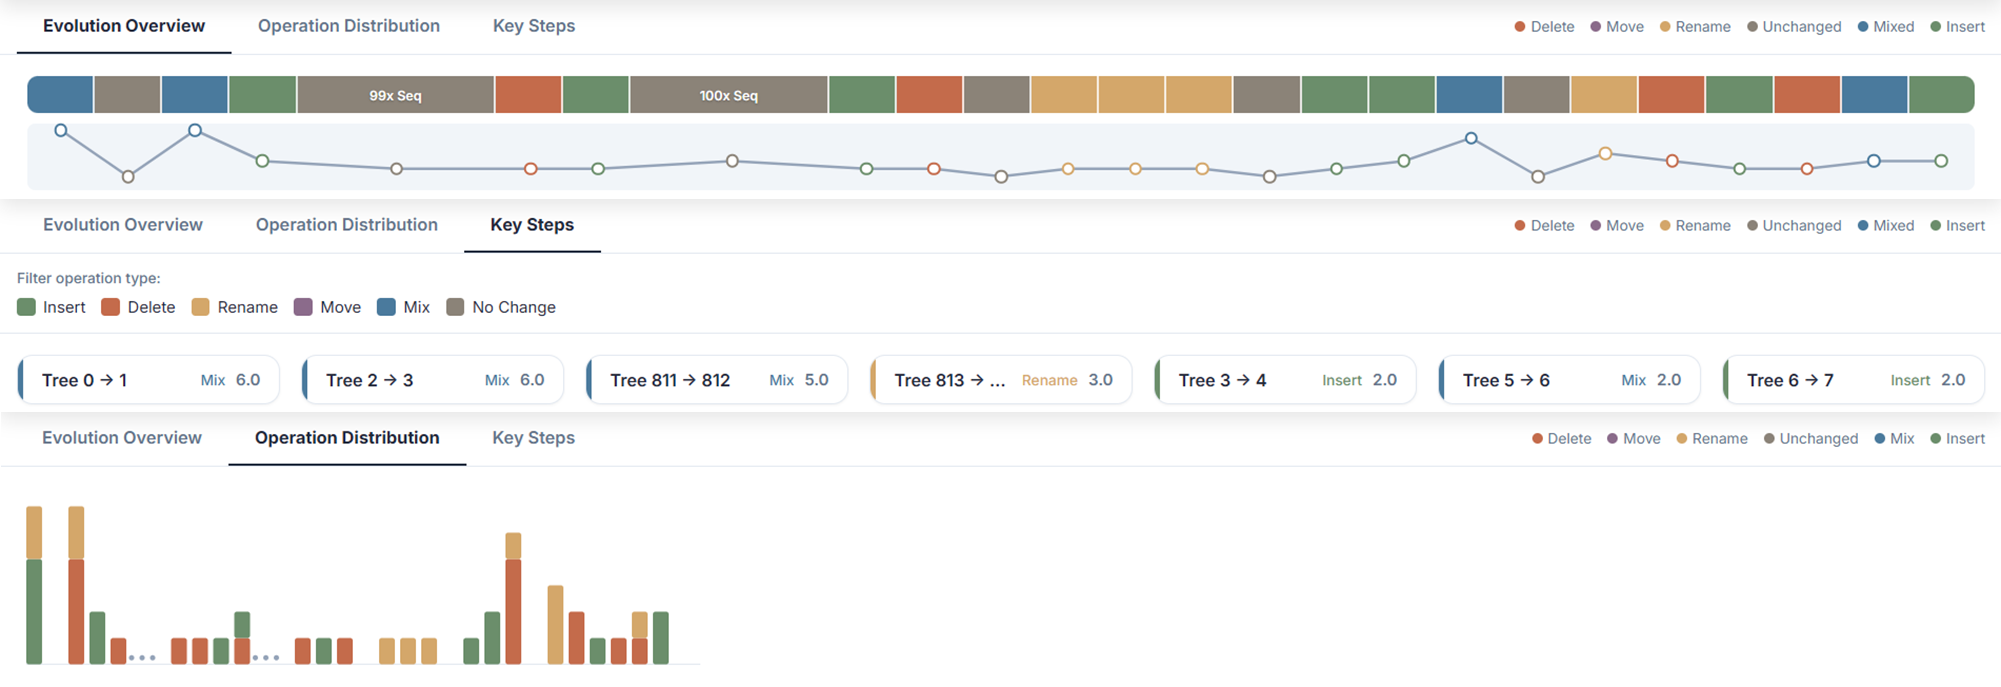
\includegraphics[width=0.9\linewidth]{figs/vis/Temp.png}

	\caption{Temporal view}
	\label{fig:temp}

\end{figure}



The statistics view provides the global entry point for temporal analysis, shown as Fig.~\ref{fig:temp}. Its main purpose is to summarize how structural change is distributed along the evolution sequence, allowing analysts to first understand the overall process before inspecting individual trees or local edits. Instead of presenting every evolution step with equal emphasis, the statistics view highlights the relative intensity, frequency, or concentration of structural changes over time, thereby helping users quickly identify salient intervals and potential transition points.

To support this goal, the statistics view encodes time-oriented summary measures derived from adjacent-tree differencing, such as change magnitude, the number of difference nodes, or the distribution of difference-aware structures across steps. These summaries give analysts a compact overview of whether the sequence evolves smoothly, exhibits abrupt transitions, or contains repeated bursts of activity. The view therefore directly supports sequence-level summarization and salient transition identification by revealing where analysts should focus their attention in long evolution sequences.

The statistics view also serves as the primary mechanism for temporal selection. Analysts can choose a contiguous time interval based on the observed summaries and pass the selected region to the downstream views. This interaction follows the \emph{zoom and filter} stage of the visual analysis process: the statistics view first presents the global context, and then guides analysts toward a subset of steps that merit more detailed structural investigation.

\subsection{Hierarchy View}
\label{sec:hierarchy_view}
\begin{figure}
	\centering
	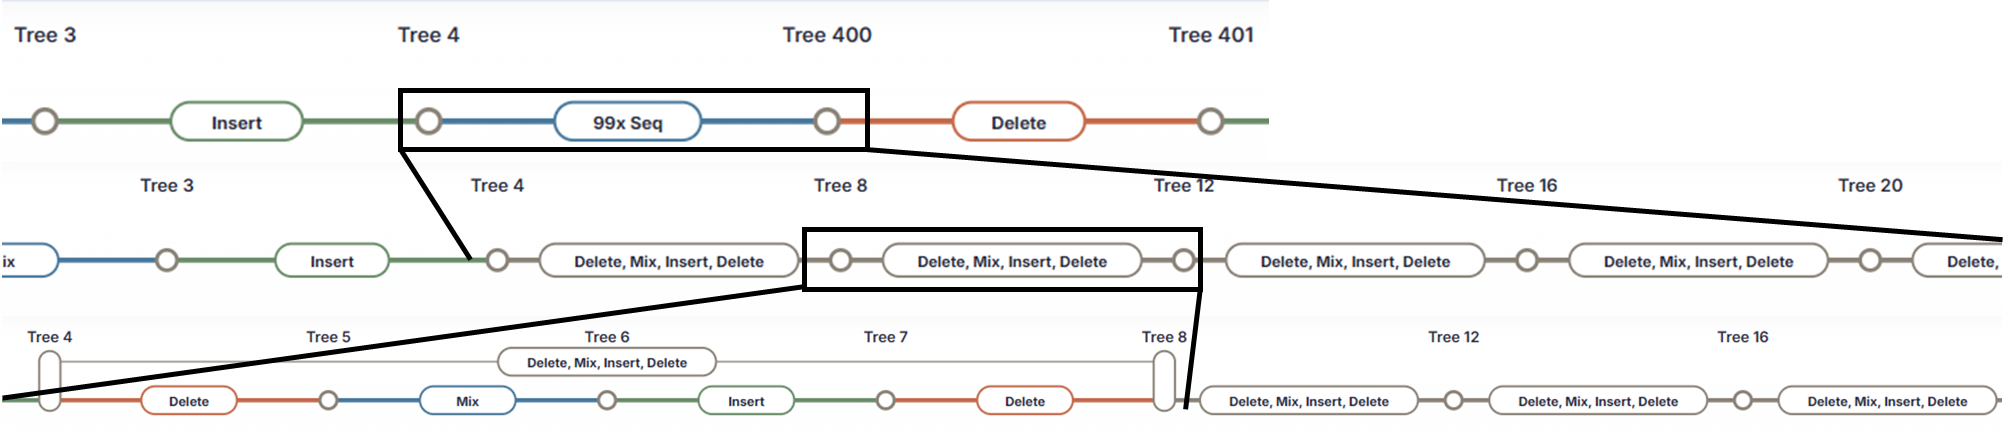
\includegraphics[width=0.9\linewidth]{figs/vis/Hierarchy.png}
	\caption{Temporal view}
	\label{fig:hierarchy}
	
\end{figure}

After a time interval is selected in the statistics view, the hierarchy view, shown as Fig.~\ref{fig:hierarchy}, provides an intermediate-level overview of the corresponding evolution region. Its role is not to expose all node-level details immediately, but to organize the selected steps into a structured representation that preserves the major hierarchical relationships among changes. In this sense, the hierarchy view acts as the bridge between global temporal summarization and detailed structural inspection.

The hierarchy view visualizes the evolution sequence within the selected interval in a compact form and supports multi-granularity analysis of changed regions. Built upon the MDF representation, it allows analysts to examine how local edits aggregate into larger structural units and how these units evolve across multiple steps. This intermediate abstraction is particularly important when changes are scattered across different parts of the tree: it helps analysts reason about whether these edits belong to the same evolving branch, correspond to repeated revisions, or indicate multiple independent transformation regions.

By presenting change structures at multiple levels of granularity, the hierarchy view supports context-preserving exploration. Analysts can inspect the selected interval at a coarse level to understand the overall structural organization of the changes, and then progressively refine their focus toward smaller substructures of interest. This view therefore supports both cross-step tracing and localized exploration while avoiding the clutter that would arise from showing all detailed trees at once.

\subsection{Tree Views}
\label{sec:tree_views}
\begin{figure}
	\centering
	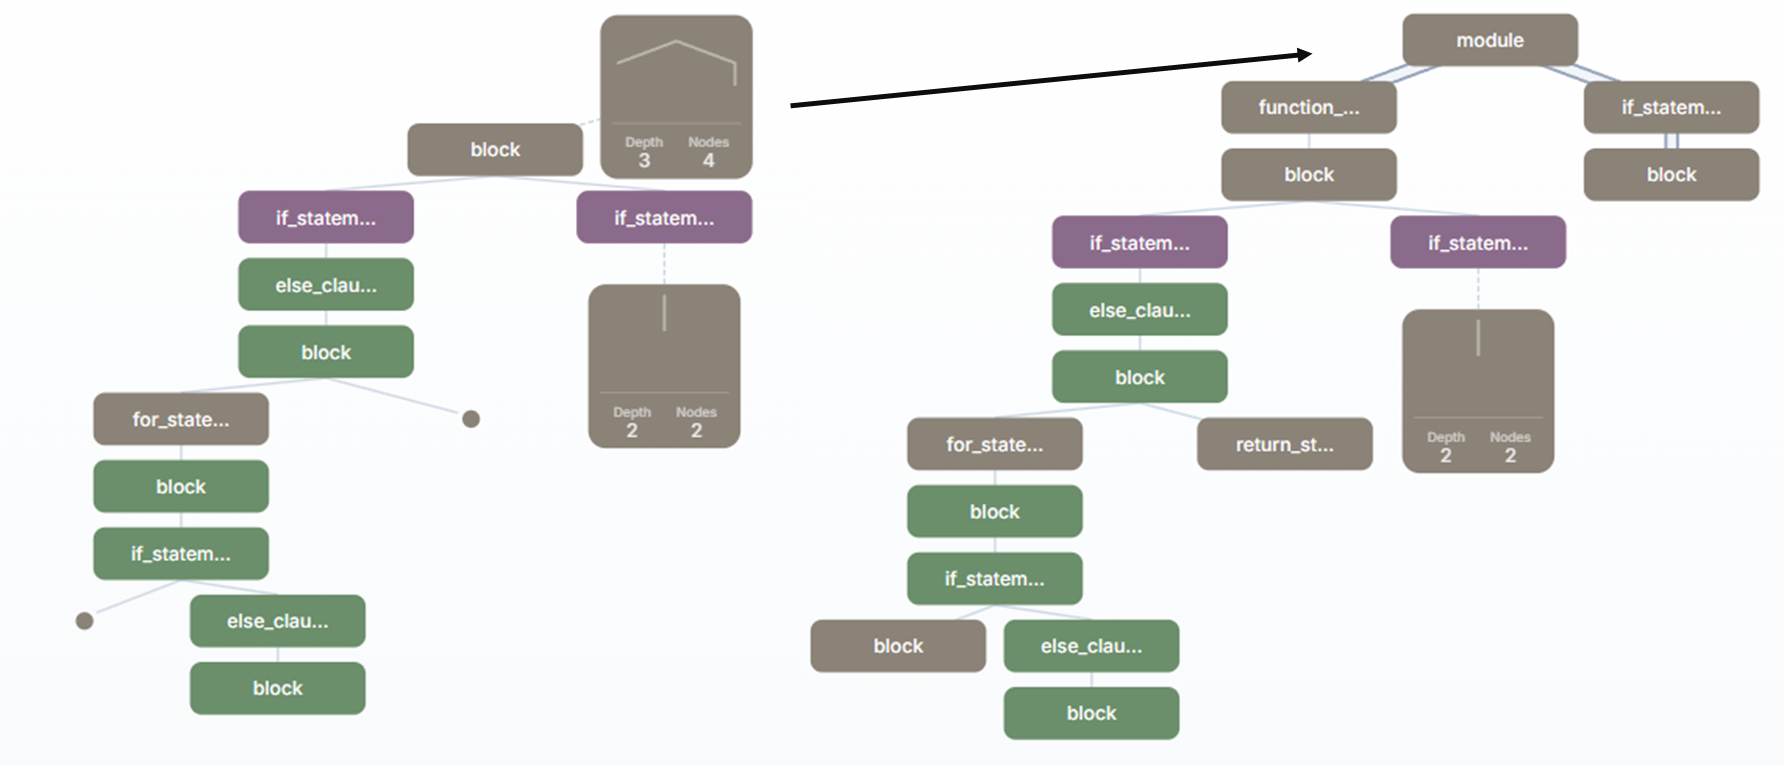
\includegraphics[width=0.9\linewidth]{figs/vis/tree.png}
	\caption{Tree view}
	\label{fig:tree}
	
\end{figure}

The tree views (shown as Fig.~\ref{fig:tree}) occupy the bottom portion of the interface and provide details on demand. While the statistics view summarizes temporal patterns and the hierarchy view organizes changes at an intermediate level, the tree views preserve the finest-grained structural information of the selected trees. They allow analysts to inspect the original tree topology, identify exact node-level edits, and verify hypotheses formed from the higher-level views.

Each tree view presents a detailed tree structure together with the local differences associated with a selected step or structural region. Through this design, analysts can examine concrete edit operations such as insertion, deletion, or move/update, and understand how these operations are embedded within the surrounding unchanged topology. The preservation of detailed context is essential because isolated change markers are often insufficient for interpretation; analysts need to see both the edit itself and its structural neighborhood.

The tree views are coordinated with the hierarchy view and the statistics view. Selections made at higher levels narrow down which trees and which structural regions are displayed in detail, while observations from detailed inspection can be traced back to their broader temporal and hierarchical contexts. In addition, we draw linking lines across adjacent trees: when analysts hover over a node, unchanged corresponding nodes in the neighboring trees are connected, allowing users to visually trace how a node is simplified or preserved across steps. This coordination allows analysts to move flexibly between overview and detail without losing orientation, thereby supporting efficient exploration of both local edits and long-range evolutionary patterns.

\subsection{Interactions}
\label{sec:vis_interactions}

The three views are linked through a set of coordinated interactions that support progressive exploration. Analysts begin with the statistics view to identify salient intervals in the temporal sequence, then select a time range for focused analysis. The hierarchy view summarizes the selected interval and allows users to inspect changed regions at different levels of granularity. Finally, the tree views reveal the detailed structures associated with selected steps or subregions.

This interaction design supports a natural analysis workflow: analysts first obtain a global overview of temporal dynamics, then filter the sequence to a region of interest, and finally inspect detailed structures on demand. Because selections are propagated across views, the interface maintains context during transitions between levels of abstraction. As a result, analysts can connect individual edits to larger structural units and relate these units back to sequence-level temporal patterns.
